\documentclass[11pt]{article}
\usepackage[utf8]{inputenc}
\usepackage[T1]{fontenc}
\usepackage[margin=1in]{geometry}
\usepackage{amsmath,amssymb}
\usepackage{booktabs}
\usepackage{graphicx}
\usepackage{xcolor}
\usepackage{xspace}
\usepackage{authblk}
\usepackage[numbers,round]{natbib}
\usepackage[hidelinks]{hyperref}
\graphicspath{{figures/}}

\newcommand{\Rope}{RoPE\xspace}
\newcommand{\M}{\ensuremath{M}\xspace}
\newcommand{\dirfrac}{\texttt{dir\_frac}\xspace}
\newcommand{\rif}{\texttt{rope\_imag\_frac}\xspace}

\title{\textbf{Steering Is Cheaper Than Banning:\\
Assistance-Based Selection of Attention's Spectral Solutions}}
\author[1]{Li Hengyu}
\affil[1]{Institute for Solid State Physics, The University of Tokyo\\
\texttt{lihengyu@issp.u-tokyo.ac.jp}}
\date{}

\begin{document}
\maketitle

\begin{abstract}
A companion study showed that the positional scheme sets the \emph{default} spectral algebra of the attention
solutions a transformer learns --- rotational (RoPE) vs.\ content-like (learned-absolute) previous-token heads ---
and that this default is a training \emph{preference}, not a hard constraint: constraints that ban a spectral
channel are rerouted around at a significant, quantifiable search cost (up to $2.9\times$ slower formation). Here we
ask the constructive converse: can pure \emph{assistance} --- initialization or regularization toward a chosen
spectral algebra, with no bans --- accelerate or \emph{select} which functionally-equivalent implementation a
circuit forms? On a controlled induction task (2-layer models, two positional schemes, $n{=}5$ seeds,
pre-registered), we find three things. (1) \textbf{Solution-specific initialization accelerates formation} in both
schemes ($-28\%$ RoPE, $-37\%$ APE; rank-biserial $+1.0$, $p{=}0.004$) at zero capability cost, whereas
initializing merely the algebra \emph{class} does not, and regularizing toward the default \emph{slows} formation
monotonically --- assistance is a property of solution-specific seeds, not of spectral fields. (2) \textbf{Weak
assistance selects the implementation}: pushed toward the non-default spectral form, $5/5$ runs form the
non-default implementation vs.\ $0/5$ free, in both schemes (Fisher $p{=}0.004$), at full capability --- and a
dissection shows the weak regularizer alone is the \emph{selector} (flipping at zero formation cost under \Rope)
while initialization alone is the \emph{accelerator}. (3)
\textbf{Steering is cheaper than banning}: the same implementation flip that costs $2.9\times$ to force by
constraint is bought by assistance at $1.3\times$ --- and the assistance cost tracks the \emph{target's} intrinsic
search difficulty (negative for RoPE's near-parity alternative, $+30\%$ for APE's hard symmetric target). We frame
these as an early, toy-scale demonstration that the spectral economy of attention is not only measurable but
\emph{steerable}, and state the open mechanism (planted RoPE rotations act as scaffolds, not seeds) and scale
caveats plainly.
\end{abstract}

\section{Background and question}
The companion paper \citep{li2026fingerprint} establishes, across seven pretrained models and three positional
schemes, that the complex spectrum of the QK operator $\M{=}W_q^\top W_k$ is the \emph{fingerprint} of the
algorithm a head implements: previous-token heads are spectrally rotational under \Rope and content-like under
learned-absolute/ALiBi positions; the profile is consolidated \emph{after} circuit formation; and constrained
training reroutes around any banned spectral channel at a significant search cost (formation-time penalty up to
$2.9\times$; all pre-registered contrasts $q_{\mathrm{BH}}{\le}0.016$). That established a \emph{negative} lever:
banning is possible but expensive and reroutable. This note tests the \emph{positive} lever --- assistance --- and
asks whether the same spectral economy that prices bans also prices, and enables, \emph{steering}.

Concretely: (Q1) does assistance toward a scheme's default algebra \emph{accelerate} circuit formation? (Q2) does
weak assistance toward the \emph{non-default} algebra \emph{select} which of two functionally-equivalent
implementations forms, without bans? (Q3) how does the cost of steering compare to the cost of banning the same
outcome? Predictions were frozen before runs (P-A1/P-A2/P-A3 in the program's roadmap); we report falsified
predictions with the same prominence as confirmations.

\section{Setup}
We reuse the companion paper's constrained-training harness: 2-layer attention-only models ($d{=}128$, 4 heads,
$d_k{=}32$) trained from scratch on a per-sequence random-map induction task (successor prediction requires
finding the previous occurrence of the current token and copying), $n{=}5$ seeds, formation step defined as the
first eval crossing the induction-CE threshold (verbatim from the companion). Free (unassisted) arms reproduce the
companion's numbers exactly ($600{\pm}0$ APE, $940{\pm}55$ RoPE). Assistance comes in three forms, all
\emph{ban-free}: (i) \emph{solution-init} --- initialize the seed heads' QK factors to carry the target
implementation's positional offset (RoPE: the $\Delta{=}{-}1$ phase $\theta$; APE: a symmetric nearby-position
plant); (ii) \emph{algebra-init} --- initialize only the target's algebra \emph{class} (random phases / a skew
plant) without the specific offset; (iii) \emph{assist-reg} --- a bounded complement penalty pushing the
population's mean spectral share toward the target, with detached denominators. Placebos apply the cross-scheme
algebra (RoPE-style under APE and vice versa) and a random orthogonal plant. Implementation class is read out by
the companion's weight batteries (\rif for RoPE, \dirfrac for APE) with thresholds pre-set from the companion's
bimodal distributions. All outputs and per-run tables are released.

\section{Results}
\textbf{(1) Assistance accelerates --- but only as solution-specific initialization.} Figure~\ref{fig:m12} and
Table~\ref{tab:m12}: solution-init speeds formation in both schemes (RoPE $940{\to}680$, $-28\%$; APE
$600{\to}380$, $-37\%$; one-sided exact MWU $p{=}0.004$, rank-biserial $+1.0$), at \emph{zero} capability cost
(final induction CE unchanged; the solution-init arms end with \emph{higher} previous-token scores). The
pre-registered primary prediction P-A1 --- that initializing the algebra \emph{class} suffices --- is
\textbf{falsified as frozen}: algebra-init is non-significant in both schemes (RoPE $q_{\mathrm{BH}}{=}0.16$,
suggestive rb$=+0.64$; APE null at the eval-grid resolution). Placebos are null (P-A2 passes): no cross-scheme or
random plant speeds formation, so the effect is target-specific, not an initialization-scale artifact. A reported
surprise: \emph{assist-reg} toward the default \emph{slows} formation, monotonically in $\lambda$ (up to $3.9\times$
at APE $\lambda{=}10$, with capability damage) --- mirroring the companion's constraint-cost law from the opposite
sign. \emph{Any global spectral field --- toward or away from the default --- has a search cost; what accelerates
is a solution-specific seed, not a field.}

\textbf{(2) Weak assistance selects the implementation.} Pushed weakly toward the \emph{non-default} form, every
run forms the non-default implementation: $5/5$ vs.\ $0/5$ free, in \emph{both} schemes (Fisher exact
$p{=}0.004$ each; zero unclassified). Under RoPE-assist every final previous-token head is cos-only
(\rif${\in}[0.016,0.043]$, kernel peak still at $\Delta{=}{-}1$) vs.\ $5/5$ phase-carried when free
(\rif${\approx}0.52$); under APE-assist every head is symmetric (\dirfrac${\approx}0.012$) vs.\ $5/5$ antisymmetric
when free. Capability is unchanged (P-A3 selection clause passes maximally). A pre-registered dissection grid
($108$ runs) then separates the two ingredients: \emph{the weak live regularizer is the selector and the
initialization is the accelerator} --- reg-only flips the implementation $5/5$ in both schemes (under RoPE at
\emph{zero} formation cost: the formation-step multiset is identical to free), while init-only accelerates
without flipping ($0/5$ both schemes); the combined arm's cost decomposes accordingly ($\approx0$ RoPE, $+30\%$
APE, carried entirely by the selection).

\textbf{(3) Steering is cheaper than banning.} The cost of assisted selection tracks the \emph{target's} intrinsic
search difficulty, and is far below the ban cost for the same outcome. Forming RoPE's cos-only implementation costs
$-23\%$ under assistance (\emph{faster} than free) vs.\ $+36$--$52\%$ to force it by banning the phase channel
(companion); forming APE's symmetric implementation costs $+30\%$ under assistance vs.\ $2.9\times$ to force it by
banning antisymmetry. \emph{Assisted selection $\ll$ constrained rerouting for the same implementation flip}
(Table~\ref{tab:cost}). The two levers also have different cost \emph{geometries}: a $\lambda$-grid over
$33\times$ shows the ban's cost is a \emph{plateau} --- the constraint binds already at $\lambda{=}0.3$ and the
delay is $\lambda$-insensitive thereafter (the cost \emph{is} the reroute, a step function of whether the ban
binds; an earlier apparent non-monotonicity did not replicate at $n{=}5$ and is retired) --- whereas
toward-default field pressure grows monotonically and, under APE, superlinearly with capability damage.

\begin{table}[t]\centering\small
\begin{tabular}{lccc}\toprule
arm & RoPE formation & APE formation & final capability\\\midrule
free & $940{\pm}55$ & $600{\pm}0$ & floor\\
algebra-init & $840{\pm}89$ (ns) & $600{\pm}0$ (ns) & floor\\
\textbf{solution-init} & $\mathbf{680{\pm}45}$ ($-28\%$) & $\mathbf{380{\pm}45}$ ($-37\%$) & floor (higher prev)\\
assist-reg $\lambda{=}1$ & $1080{\pm}45$ (slower) & $960{\pm}55$ (slower) & floor\\
assist-reg $\lambda{=}10$ & $1380{\pm}130$ (slower) & $2340{\pm}219$ (slower) & APE damaged\\
\bottomrule\end{tabular}
\caption{Assistance-hinge formation steps ($n{=}5$; one-sided exact MWU vs.\ free, BH-FDR). Solution-specific
initialization accelerates both schemes at rank-biserial $+1.0$, $p{=}0.004$; algebra-class init and
regularization fields do not.}
\label{tab:m12}
\end{table}

\begin{table}[t]\centering\small
\begin{tabular}{lccc}\toprule
implementation flip & ban cost (companion) & \textbf{assist cost (this note)} & selection\\\midrule
$\to$ RoPE cos-only (non-default) & $+36$--$52\%$ & $\mathbf{-23\%}$ (faster) & $5/5$ vs $0/5$\\
$\to$ APE symmetric (non-default) & $2.9\times$ & $\mathbf{+30\%}$ & $5/5$ vs $0/5$\\
\bottomrule\end{tabular}
\caption{Steering vs.\ banning for the same implementation flip (Fisher $p{=}0.004$ each). Assistance selects the
same outcome a ban forces, far more cheaply; the assist cost tracks the target's intrinsic search difficulty.}
\label{tab:cost}
\end{table}

\begin{figure}[t]\centering
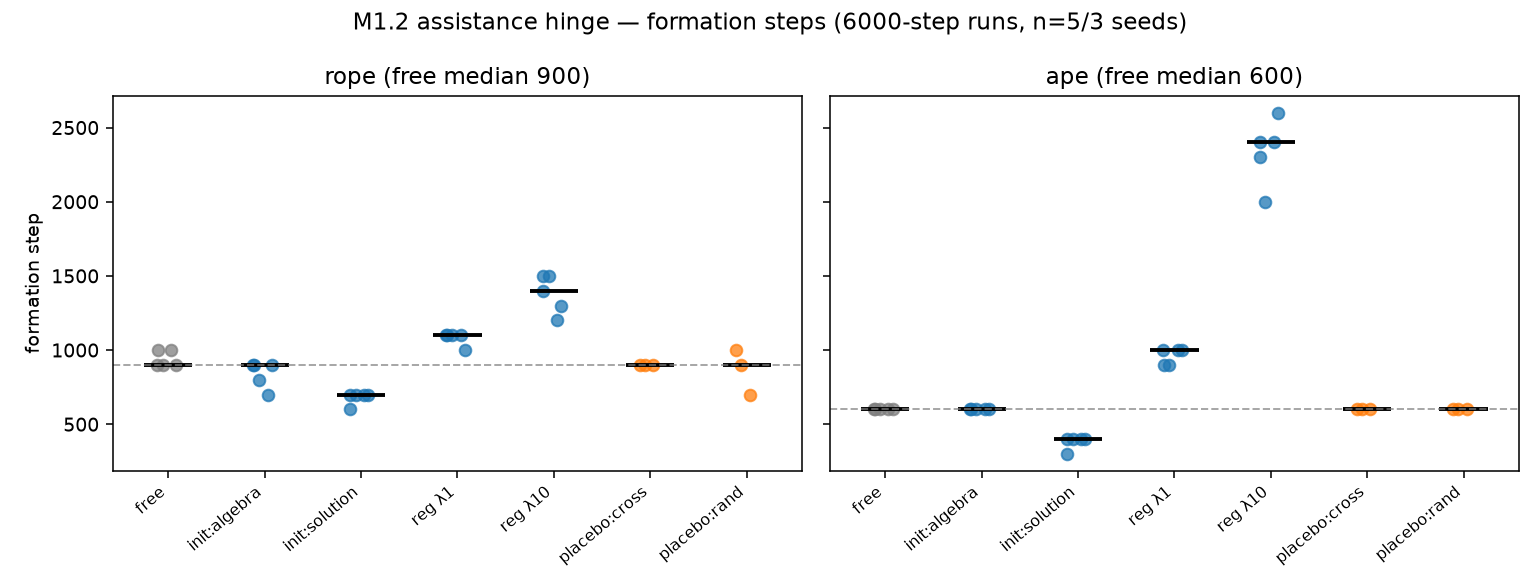
\includegraphics[width=\linewidth]{m12_formation.png}
\caption{Formation steps by assistance arm (left RoPE, right APE; $n{=}5$/3 seeds). Solution-init (third column)
accelerates both schemes; algebra-init and placebos sit at free; regularization fields slow formation, monotonically
in $\lambda$.}
\label{fig:m12}
\end{figure}

\section{Open mechanism and caveats}
\textbf{Scaffold, not seed.} Under RoPE the planted solution is \emph{never} adopted --- in all $5/5$ acceleration
runs the planted heads end with prev${\approx}0.02$ and the circuit forms in \emph{unseeded} heads --- yet
formation still accelerates $28\%$. The RoPE plant acts as a \emph{scaffold} (candidate mechanisms: gradient
shaping through the second layer / OV, or the plant's coherent structure aiding early representation formation),
not a seed. Under APE the plant \emph{is} adopted ($5/5$). A pre-registered freeze test sharpens the scaffold
reading: \emph{freezing the plant entirely} (no gradient into the seeded heads) preserves --- in fact
\emph{doubles} --- the speedup ($500$ median vs.\ $700$ unfrozen vs.\ $900$ free; rb$=+1.0$, capability intact).
The seed need not even be trainable; training's own modification of the planted heads apparently \emph{degrades}
the scaffold, pointing at a representational/gradient-shaping mechanism rather than plant adaptation --- which we
still flag as open rather than adjudicated.
\textbf{Caveats}: $n{=}5$; 2-layer attention-only models on one synthetic task; APE formation is quantized at the
$100$-step eval grid (so the APE algebra-init null means ``no effect at $100$-step resolution,'' not a measured
zero). These results are an existence demonstration of steerability at toy scale, not a scaling law. A
160M-parameter pretraining pilot (through the induction formation window) tests transfer and returns a mixed,
honestly negative-leaning early picture: the ban-induced implementation selection reproduces (the previous-token
head re-forms cos-only at 160M) with a formation-time cost of the same sign, but the solution-init
\emph{acceleration} does \emph{not} transfer (assist$-$free $\le0$ in both seeds, against the $-44\%$
frozen-scaffold speedup at toy scale), and weak-regularizer selection remains untested at scale. Formation at 160M
appears data- and optimization-limited rather than search-limited, the regime in which initialization would help.

\section{Takeaway}
The spectral economy of attention is not only measurable and priced (companion paper) but \emph{steerable} at toy
scale: weak, ban-free assistance selects which functionally-equivalent spectral implementation a circuit adopts, at
a cost far below banning the alternative, while solution-specific initialization accelerates circuit formation
(toy scale only; the acceleration does not survive at 160M, see the caveats above). To the extent selection
transfers --- our 160M pilot finds the ban-induced selection reproduces --- ``which algorithm a circuit
implements'' becomes a partly controllable design choice, relevant to interpretability-by-construction and to
installing a chosen implementation class. The one knob that transfers happens to install a
\emph{weight-audit-evading} implementation (cos-only, \rif$\,{\approx}0.003$); it is nonetheless not hideable,
because companion propagator-level work finds that implementations which vanish from the weight fingerprint remain
fully visible as transient-reserve excess on the attention propagator ($31/31$ prev-carrying heads positive across
all implementations). The weight battery reads \emph{implementation}, the propagator battery reads \emph{function},
so a steered or rerouted circuit cannot evade both. We release the harness, seeds, and per-run tables.

\paragraph{Reproducibility \& pre-registration.} Harness \texttt{src/\{h1\_hinge,h1\_analyze,h2\_m21\}.py}
(extends the companion's \texttt{p10} additively; free arms bit-exact); predictions P-A1/P-A2/P-A3 and the
follow-up family P-M21a--d/P-A5/P-E2 frozen before their respective runs; per-run tables
\texttt{results/h1/m12\_summary.parquet}, \texttt{m13\_summary.parquet}, \texttt{results/h2/}; falsified
predictions (P-A1; the $\lambda$ non-monotonicity flag P-M21c) reported as findings. Code and data:
\url{https://github.com/HengyuLi-Ozaki-lab/qk-spectral-fingerprint}.

\bibliographystyle{plainnat}
\bibliography{references}
\end{document}
